\section{Kjerneteknologi: Sivil næringsmiddelinfrastruktur}
\label{sec:kjerneteknologi}

Å frakte drikkevann til sårbare grupper og sykehus under en biologisk krise stiller strengere hygienekrav enn ordinære kommunale vannrør. Norsk meieriindustri transporterer daglig råmelk---en biologisk væske med ideelle vekstvilkår for patogener. Teknologien som sikrer råmelkens mikrobiologiske kvalitet utgjør en sovende beredskapsressurs.

\subsection{Materialteknologi og biofilmfrie overflater}
Konstruksjonen av melketankbiler skiller seg radikalt fra ordinære industritankbiler:
\begin{itemize}[leftmargin=1.5em, itemsep=0.2em]
    \item \textbf{Elektropolert syrefast stål:} Tanker og røropplegg er produsert i austenittisk rustfritt stål (\textsc{aisi} 316L / \textsc{en} 1.4404) med molybdenlegering, elektropolert til $Ra \le \SI{0.4}{\micro\meter}$. Den mikroskopiske planheten eliminerer sprekker der mikroorganismer kan hefte, hvilket gjør biofilmdannelse fysisk umulig.
    \item \textbf{Fullisolert termoskonstruksjon:} Dobbelveggede tanker isolert med høydensitets polyuretanskum (\textsc{pur}) sikrer at forhåndskjølt vann holder en stabil temperatur under \SI{6}{\celsius} gjennom transporten, selv på varme sommerdager, og hindrer bakteriell vekst.
\end{itemize}

\subsection{Autonom termisk og kjemisk sterilisering (\textsc{cip})}
Før innsats steriliseres tankbilene ved meierienes helautomatiserte og lukkede \textsc{cip}-stasjoner (\textit{Cleaning-In-Place}), som illustrert i figur~\ref{fig:cip}:
\begin{enumerate}[leftmargin=1.5em, itemsep=0.15em]
    \item \textbf{Forhåndsspyling:} Lunkent vann (\SI{45}{\celsius}) fjerner grove væskerester.
    \item \textbf{Alkalisk fase (lutvask):} \SI{2.0}{\percent} natriumhydroksid (\textsc{naoh}) ved \SI{75}{\celsius} i 10 minutter forsåper fett og hydrolyserer proteinbindinger.
    \item \textbf{Mellomspyling:} Rentvannsskylling fjerner kjemikalierester.
    \item \textbf{Syrefase:} \SI{1.5}{\percent} salpetersyre (\textsc{hno}$_3$) ved \SI{65}{\celsius} nøytraliserer baserester og løser opp mineraler og melkestein.
    \item \textbf{Termisk sterilisering:} Avsluttende overopphetet vann og damp ved $\ge \SI{85}{\celsius}$ i 15 minutter.
\end{enumerate}

Prosessen overvåkes kontinuerlig av sensorer for ledningsevne, turbiditet og temperatur. Digital vaskelogg verifiserer $\log 6$-reduksjon (\num{99.9999}\% reduksjon) av patogener.

\begin{figure}[htbp]
    \centering
    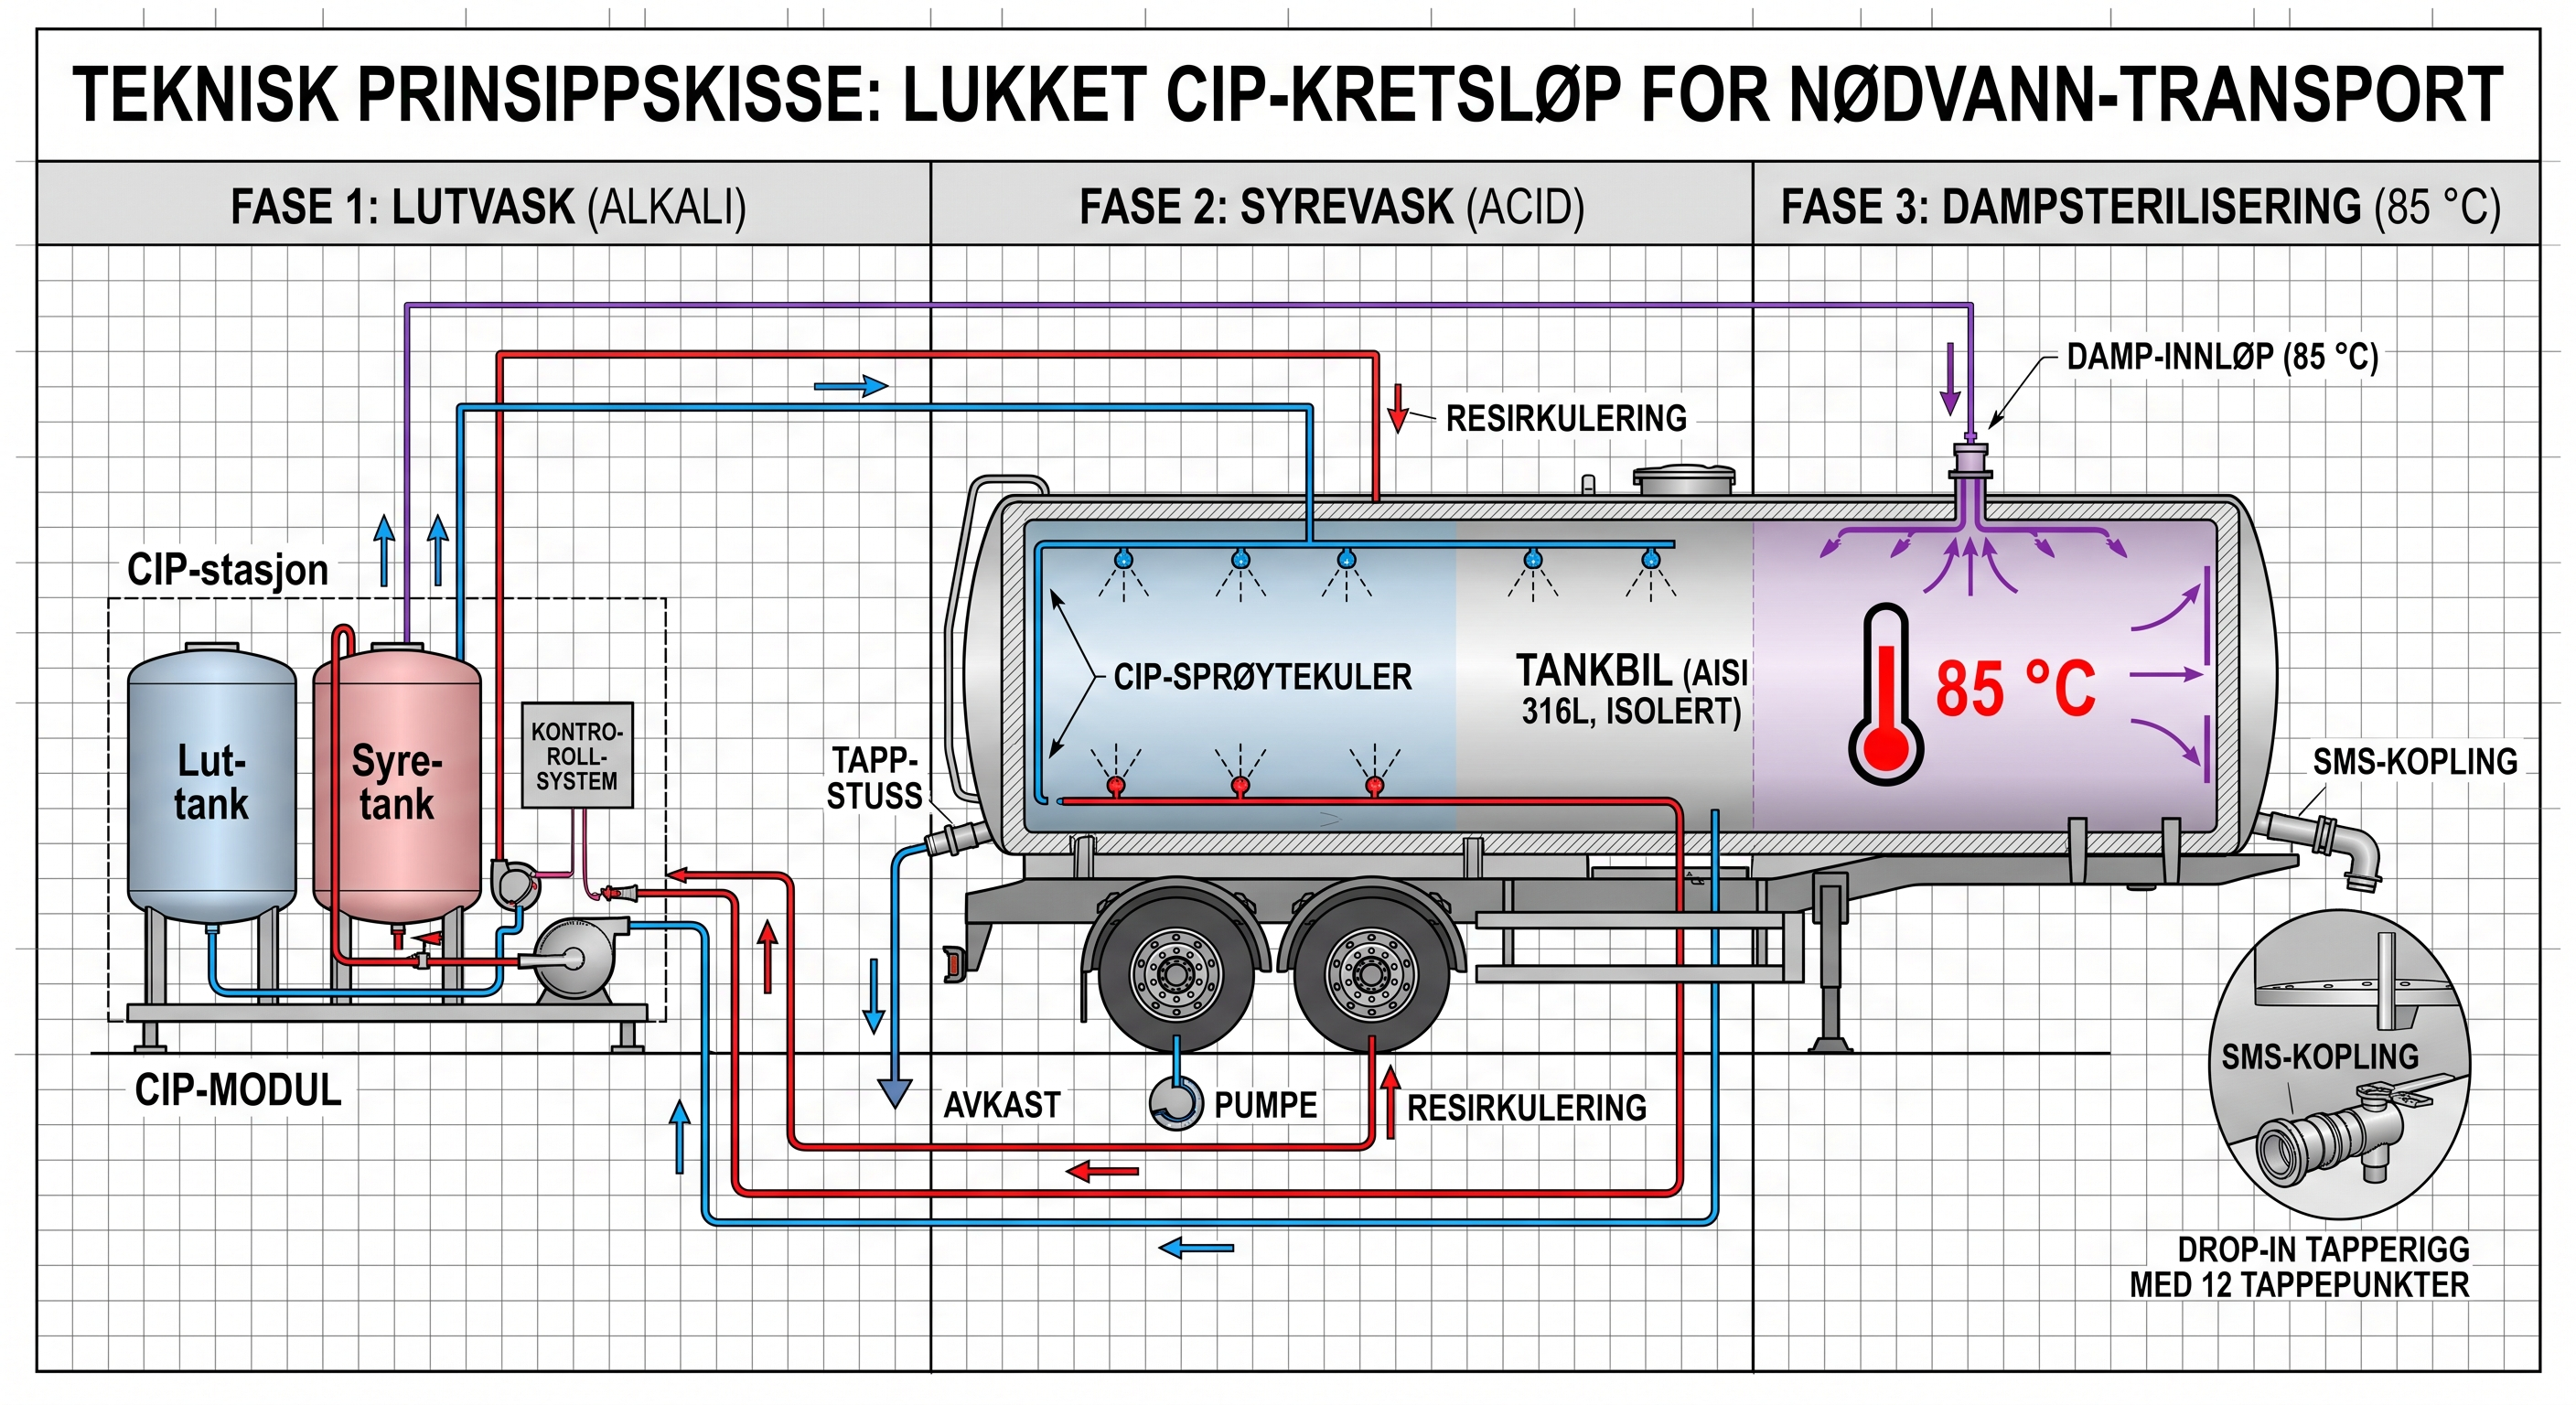
\includegraphics[width=0.92\textwidth]{Figures/CIP-process.jpg}
    \caption{Skjematisk oversikt over den automatiserte \textsc{cip}-vaskesyklusen. Vekslingen mellom termisk energi, lut og syre garanterer kjemisk renhet og bakteriologisk sterilitet.}
    \label{fig:cip}
\end{figure}

\subsection{Håndtering av melkeproteiner og allergenbarrierer}
Alvorlig melkeallergi mot kasein eller myseprotein ($\beta$-laktoglobulin) kan utløse anafylaksi hos spedbarn og pasienter. Prosjekt Meierikjeden etablerer derfor en uavhengig allergenbarriere basert på kjemisk degradering og to-trinns feltverifisering:
\begin{enumerate}[leftmargin=1.5em, itemsep=0.15em]
    \item \textbf{Alkalisk hydrolyse:} Varm lutvask (\SI{2.0}{\percent} \textsc{naoh}, \SI{75}{\celsius}, $\text{pH} > 12.5$) spalter melkeproteinenes peptidbindinger irreversibelt og denaturerer de immunogene epitopene.
    \item \textbf{To-trinns feltverifisering før fylling:}
    \begin{itemize}[leftmargin=1.5em, itemsep=0.1em]
        \item \textit{\textsc{atp}-bioluminescens:} Svaberprøve analyseres på 30 sekunder; måleverdier under 10 \textsc{rlu} bekrefter fravær av organisk restmateriale.
        \item \textit{Lateral-flow hurtigteststrips:} Immunokromatografiske strips dyppes i skyllevannet. Deteksjonsgrensen på $< \SI{1}{ppm}$ (\SI{1}{\micro\gram\per\milli\liter}) gir visuelt svar innen 5 minutter.
    \end{itemize}
\end{enumerate}
Vann fylles først når begge tester er negative, hvilket garanterer null allergirisiko.

\subsection{Hydraulisk kapasitet og lukkede kretsløp}
Hver tankbil rommer \num{15000} til \SI{25000}{\liter} og disponerer sanitære impellerpumper i syrefast stål (\SI{1000}--\SI{1500}{\liter\per\minute}). En tank på \SI{20}{\cubic\meter} fylles eller tømmes dermed på under 20 minutter. Utlufting skjer gjennom sterile \textsc{hepa}-luftfiltre for å hindre luftbåren kontaminering.
